%----------------------------------------------------------------------------------------
%   PACKAGES AND OTHER DOCUMENT CONFIGURATIONS
%----------------------------------------------------------------------------------------

\documentclass[fleqn,10pt]{SelfArx} % Document font size and equations flushed left

\setlength{\columnsep}{0.55cm} % Distance between the two columns of text
\setlength{\fboxrule}{0.75pt} % Width of the border around the abstract

\definecolor{color1}{RGB}{0,0,90} % Color of the article title and sections
\definecolor{color2}{RGB}{0,20,20} % Color of the boxes behind the abstract and headings

\newlength{\tocsep} 
\setlength\tocsep{1.5pc} % Sets the indentation of the sections in the table of contents
\setcounter{tocdepth}{3} % Show only three levels in the table of contents section: sections, subsections and subsubsections

\usepackage{lipsum} % Required to insert dummy text
\usepackage{lastpage} %last page
\usepackage{hyperref} % For hyperlinks
\usepackage{url} % For hyperlinks

%----------------------------------------------------------------------------------------
%   ARTICLE INFORMATION
%----------------------------------------------------------------------------------------

\JournalInfo{Multivariate Time Series and Financial Econometrics, No. 1, 1-\pageref{LastPage}, 2025} 
\Archive{} % Additional notes (e.g. copyright, DOI, review/research article)

\PaperTitle{Multivariate Time Series Analysis of Air Quality Data in Delhi} % Article title

\Authors{Aleksandr Jan Smoliakov \textsuperscript{1}*}
\affiliation{\textsuperscript{1}\textit{Department of Econometric Analysis, Faculty of Mathematics and Informatics, Vilnius University}} % Author affiliation
\affiliation{*\textbf{Corresponding author}: aleksandr.smoliakov@mif.stud.vu.lt} % Corresponding author

\Keywords{air pollution --- multivariate time series --- VAR --- VARMA --- forecasting} % Keywords - if you don't want any simply remove all the text between the curly brackets
\newcommand{\keywordname}{Keywords} % Defines the keywords heading name

%----------------------------------------------------------------------------------------
%   ABSTRACT
%----------------------------------------------------------------------------------------

\Abstract{This project blueprint outlines an investigation into the application of multivariate time series models, inspired by techniques from financial econometrics, to forecast the air quality in Indian cities. Using daily measurements of five pollutant concentrations in Delhi collected between 2018 and 2019, the study will aim to assess the temporal dynamics between pollutants. The discussed methodologies will form the foundation for subsequent steps involving data transformation, model estimation, and interpretation of forecasting results. Specifically, this report focuses on a detailed analysis of five key pollutants ($PM_{2.5}$, $PM_{10}$, $NO_{2}$, CO, $NH_{3}$) in Delhi for the period 2018-2019, employing VAR and VARMA models to understand their interdependencies and to generate forecasts.}

%----------------------------------------------------------------------------------------

\begin{document}

\flushbottom % Makes all text pages the same height

\maketitle % Print the title and abstract box

\tableofcontents % Print the contents section

\thispagestyle{empty} % Removes page numbering from the first page

%----------------------------------------------------------------------------------------
%   ARTICLE CONTENTS
%----------------------------------------------------------------------------------------

\section*{Introduction} % The \section*{} command stops section numbering

\addcontentsline{toc}{section}{\hspace*{-\tocsep}Introduction} % Adds this section to the table of contents with negative horizontal space equal to the indent for the numbered sections

Urban air quality is a critical public health and environmental issue, especially in rapidly urbanizing regions. Accurate forecasting of air quality indicators, such as pollutant (e.g., $PM_{2.5}$, $PM_{10}$, $NO_{2}$, CO) concentrations and their composite measures like the Air Quality Index (AQI), is essential for formulating timely policy interventions.

While univariate models (e.g., ARIMA) offer a baseline for prediction, complex datasets with interconnected variables require the advanced analytical capabilities of multivariate time series models. In financial econometrics, multivariate approaches -- such as vector autoregression (VAR) and vector autoregressive moving average (VARMA) models -- have been used to model the interdependencies among multiple time series, capturing interactions between variables and their lagged effects. These methodologies could be equally applicable to environmental datasets where pollutant concentrations interact over time.

In this project, I propose to analyze the \emph{Air Quality Data in India (2015--2020)} dataset, which contains hourly observations of twelve pollutant concentrations (as well as the Air Quality Index, AQI) measured in 20 Indian cities. Specifically, I will use daily-aggregated data from Delhi, which has been identified as one of the most polluted cities in the world. The focus will be on five key pollutants: Particulate Matter ($PM_{2.5}$, $PM_{10}$), Nitrogen Dioxide ($NO_2$), Carbon Monoxide ($CO$), and Ammonia ($NH_3$), covering the period from January 1, 2018, to January 1, 2020.

The objective of this project is to apply multivariate models to capture the dynamic interactions among these pollutants in Delhi and provide robust air quality forecasts. This involves data preprocessing, stationarity testing, VAR and VARMA model estimation, Granger causality analysis, impulse response analysis, forecast error variance decomposition, and forecast evaluation.

%------------------------------------------------

\section{Literature Review}
Recent studies on air quality forecasting have adopted various time series modeling techniques, ranging from univariate to multivariate approaches. This section reviews relevant contributions in the field, focusing on the strengths and limitations of different methodologies.

\subsection*{Analysis of Air Quality using Univariate and Multivariate Time Series Models}
Sethi and Mittal (2020) investigate the prediction of daily Air Quality Index (AQI) values in Gurugram, India by comparing univariate and multivariate time series methods \cite{sethi2020}. Using ARIMA and VAR models, they demonstrate that, for their dataset, a simpler univariate ARIMA model gives more accurate predictions of AQI than the multivariate counterpart. The authors conclude that multivariate VAR models faced instability in handling the additional noise introduced by interdependent pollutant series. This paper provides valuable insights on the challenges of multivariate data modeling, especially the impact of differencing and parameter selection on model stability.

\subsection*{Multivariate Time Series Modelling for Urban Air Quality}
Hajmohammadi and Heydecker (2021) focus on urban air quality forecasting in multiple meteorological stations in London \cite{hajmohammadi2021}. The authors compare seasonal ARMA (SARMA) models with vector ARMA (VARMA) models, which account for both spatial and temporal dependencies. The study demonstrates that while SARMA models capture individual station trends, VARMA outperforms it by accounting for cross-station interactions. The findings emphasize that in complex urban environments, accounting for spatial interactions can significantly enhance predictive performance. This concept could be applicable for modeling pollutant interdependencies in the larger-scale Indian context.

\subsection*{Forecasting of Particulate Matter with a Hybrid ARIMA Model Based on Wavelet Transformation and Seasonal Adjustment}
Aladağ (2021) introduces a hybrid modeling approach that integrates seasonal adjustment, wavelet transformation, and ARIMA \cite{aladag2021}. Applied to forecasting PM10 in Erzurum, Turkey, this method combines a classical ARIMA model with wavelet decomposition, capturing both low-frequency trends and high-frequency variations present in the pollutant time series. This study provides a method for addressing seasonality and nonstationarity -- features also present in air quality data -- by decomposing the series before reassembling the forecasted components.

\medskip

The insights from these studies suggest the use of multivariate frameworks in forecasting. Techniques from financial econometrics are shown to be effective when adapted to environmental datasets. Advanced data transformation methods, such as wavelet decomposition, can also enhance model performance. The project will thus build on these methodologies to analyze the air quality data in India.

%------------------------------------------------

\section{Methodology}
This section outlines the data source, preparation steps, and the multivariate time series models to be used in the analysis. The focus will be on the application of VAR and VARMA models to capture the interdependencies among pollutants and generate forecasts in Delhi.

The analysis was conducted using the R~\cite{RCoreTeam2025} programming language and the following packages: \texttt{dplyr}~\cite{dplyr}, \texttt{ggplot2}~\cite{ggplot2}, \texttt{tidyr}~\cite{tidyr}, \texttt{forecast}~\cite{forecast}, \texttt{urca}~\cite{urca}, \texttt{vars}~\cite{vars}, and \texttt{MTS}~\cite{MTS}.

\subsection{Data Source and Preparation}
The raw dataset \textit{Air Quality Data in India (2015--2020)} contains hourly measurements of multiple pollutants across 20 Indian cities. For this project, I selected data for five key pollutants: Particulate Matter ($PM_{2.5}$, $PM_{10}$), Nitrogen Dioxide ($NO_2$), Carbon Monoxide ($CO$), and Ammonia ($NH_3$).

The period of interest is from January 1, 2018, to January 1, 2020, covering two full years of data. The decision to focus on Delhi and this specific time frame is based on the better availability and quality of data for Delhi in the selected period.

\subsubsection{Missing Value Imputation}
An initial analysis of the dataset revealed a significant number (10-40\%) of missing values in the majority of the cities data. Delhi exhibited the least amount of missing data, with under 1\% of the values missing. Given its completeness and significance, Delhi was chosen as the focus for this detailed multivariate analysis.

To address the missing values in the dataset, a linear interpolation method using the \texttt{na.interp} function from the \texttt{forecast} package was used. This method estimates missing values based on the surrounding data points, ensuring a smooth transition between known values. The imputation process was applied to each pollutant series separately.

\subsubsection{Data Transformation}
Pollutant concentration data is non-negative and exhibits significant right-skewness and non-constant variance. To address this, a $\log(x+1)$ transformation (log1p) was applied to each pollutant series. This transformation stabilizes variance and normalizes the distribution, making it more suitable for time series modeling. The 1 added to the data ensures that the logarithm is defined for all values, including zero.

\subsubsection{Data Aggregation}
While the dataset contains hourly measurements, modelling data of such granularity may be difficult due to noise, overlapping seasonal patterns, and the computational challenge of handling large, high frequency time series datasets. The hourly data was aggregated to daily frequency by taking the mean of the log1p-transformed values for each day. This aggregation reduces noise while preserving the underlying patterns in daily pollutant concentrations. The resulting daily time series covered 732 observations for each pollutant.

\subsection{Exploratory Data Analysis}
Exploratory Data Analysis (EDA) was performed on the log1p-transformed and aggregated data to understand the underlying patterns, trends, and seasonality in the time series. The EDA included:
\begin{itemize}
    \item Time series plots to visualize the trends and seasonality in each pollutant series.
    \item A correlation matrix and its visualization using \texttt{corrplot} was generated to assess the same-day linear correlations between pollutants.
\end{itemize}

\subsection{Stationarity Testing}
Stationarity is a necessary assumption for many time series models. To assess the stationarity of each pollutant series, Augmented Dickey-Fuller (ADF) test was used (\texttt{ur.df} function from the \texttt{urca} package). The null hypothesis of the ADF test is that the time series has a unit root, indicating non-stationarity. AIC criterion was used to select the optimal lag order for the ADF test, and the test was performed at a significance level of 0.05. If the null hypothesis is rejected, the series can be considered stationary.

\subsection{Multivariate Time Series Models}
Based on stationarity test results, appropriate multivariate models were selected.
\subsubsection{Vector Autoregression (VAR) Model}
If the time series are found to be stationary (I(0)), a VAR model can be directly applied. A VAR(p) model expresses each variable as a linear function of its own past $p$ values and the past $p$ values of all other variables in the system.
\begin{equation}
Y_t = c + A_1 Y_{t-1} + \cdots + A_p Y_{t-p} + \epsilon_t
\end{equation}
where \(c\) is a constant vector, \(Y_t\) is a vector of the time series variables at time \(t\), \(A_i\) are the coefficient matrices, \(p\) is the lag order, and \(\epsilon_t\) is a vector of error terms.
The VAR model can be estimated using the \texttt{VAR} function from the \texttt{vars} package in R. The optimal lag order $p$ was determined using the Akaike Information Criterion (AIC), provided by the \texttt{VARselect} function. The VAR model was fitted using the \texttt{VAR} function.

\subsubsection{Vector Autoregressive Moving Average (VARMA) Model}
VARMA models extend VAR models by including moving average (MA) terms. This allows for capturing both the autoregressive and moving average structures in the data. The VARMA model is suitable for stationary data. A VARMA(p,q) model can be expressed as:
\begin{equation}
Y_t = A_1 Y_{t-1} + A_2 Y_{t-2} + \cdots + A_p Y_{t-p} + B_1 \epsilon_{t-1} + B_2 \epsilon_{t-2} + \cdots + B_q \epsilon_{t-q} + \epsilon_t
\end{equation}
where \(B_i\) are the MA coefficient matrices, \(q\) is the order of the MA part, and \(\epsilon_t\) is a vector of error terms.
The VARMA model was estimated using the \texttt{VARMA} function from the \texttt{MTS} package in R. The optimal lag was not determined using automated methods, but rather based on model fit and performance metrics.

\subsection{Model Analysis}

The fitted VAR model was analyzed to understand the interdependencies among pollutants. The following analyses were performed:
\begin{itemize}
    \item Granger Causality Tests conducted using the \texttt{causality} function from the \texttt{vars} package to determine if past values of one pollutant significantly predict current values of another, considering all pollutants in the VAR system.
    \item Impulse Response Functions (IRFs) trace the effect of a one-standard-deviation shock to one variable on current and future values of all variables in the VAR system. These were generated using the \texttt{irf} function.
    \item Forecast Error Variance Decomposition (FEVD) shows the proportion of the forecast error variance of each variable that can be attributed to its own shocks versus shocks to other variables in the system. This was computed using the \texttt{fevd} function.
\end{itemize}

\subsection{Forecasting and Evaluation}
To evaluate forecasting performance, the daily dataset for Delhi (732 observations) was split into a training set (first 718 observations) and a test set (last 14 observations). A forecast horizon of 14 days was chosen.
Models (VAR and VARMA) were trained on the training set, and 14-step-ahead forecasts were generated. The Root Mean Squared Error (RMSE) was used to compare the forecast accuracy of the models for all five pollutants. RMSE is defined as:
\begin{equation}
\text{RMSE} = \sqrt{\frac{1}{H} \sum_{h=1}^{H} (y_{T+h} - \hat{y}_{T+h})^2}
\end{equation}
where $H$ is the forecast horizon, $y_{T+h}$ is the actual value, and $\hat{y}_{T+h}$ is the forecasted value.

%------------------------------------------------

\section{Results and Discussion}
\subsection{Data Preprocessing and EDA}
The initial dataset consisted of hourly measurements of twelve pollutants across 20 Indian cities from 2015 to 2020. For focused analysis, data from January 1, 2018 to January 1, 2020 was selected. The pollutants of interest were $PM_{2.5}$, $PM_{10}$, $NO_{2}$, CO, and $NH_{3}$.
Delhi was selected for analysis and modeling due to its relatively complete data and significance as a major urban center with severe air quality issues.
The data was preprocessed to handle missing values, which were imputed using linear interpolation. The log1p transformation was applied to stabilize variance and normalize the distribution of pollutant concentrations.
The hourly log1p-transformed data were then aggregated to daily mean values, resulting in 732 observations per pollutant for Delhi. Figure~\ref{fig:log_dist_delhi} shows the distributions of the daily mean log1p-transformed pollutant concentrations, indicating a reasonably unskewed distribution after transformation.

\begin{figure}[ht]
    \centering
    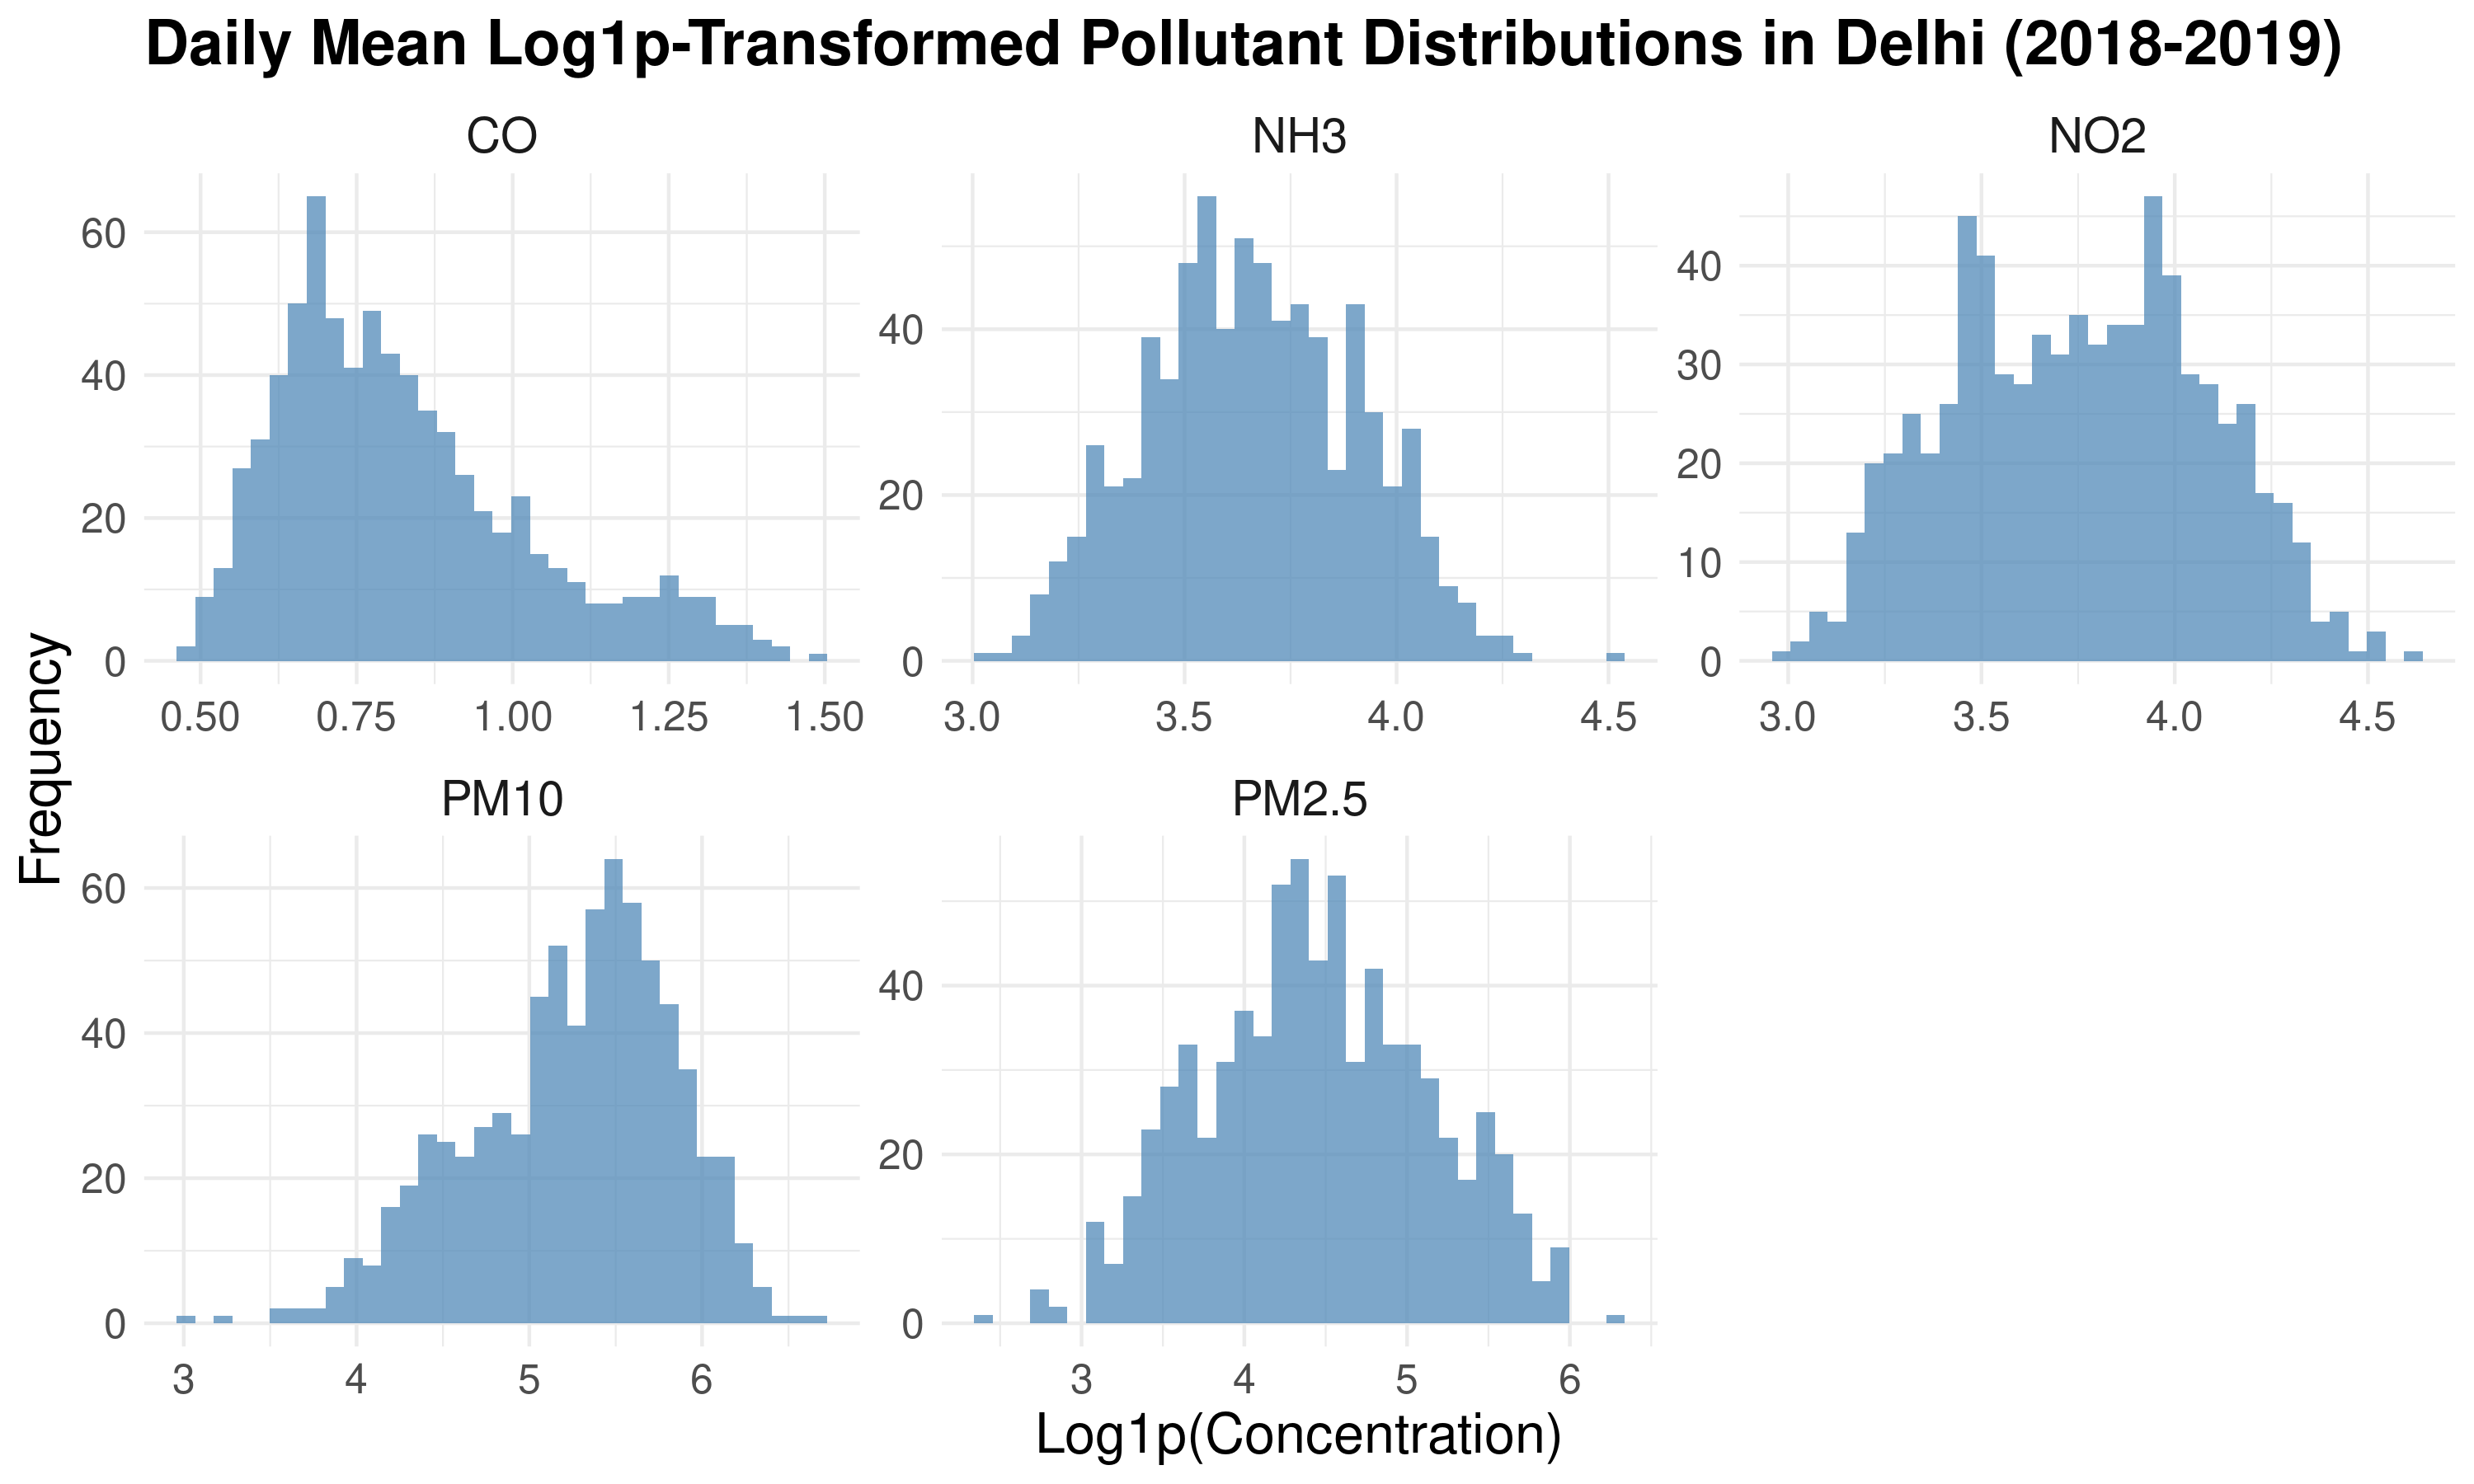
\includegraphics[width=\linewidth]{../analysis/assets/log1p_delhi_distributions.png}
    \caption{Histograms of Daily Mean log1p-Transformed Pollutant Concentrations in Delhi (2018-2019).}
    \label{fig:log_dist_delhi}
\end{figure}

\subsubsection{Time Series Behavior}
Time series plots of the daily mean log1p-transformed pollutant concentrations for Delhi are presented in Figure~\ref{fig:daily_ts_delhi}. These plots reveal noticeable patterns, including seasonality, with higher pollutant levels typically observed during winter months and lower levels during summer months.

\begin{figure*}[ht]
    \centering
    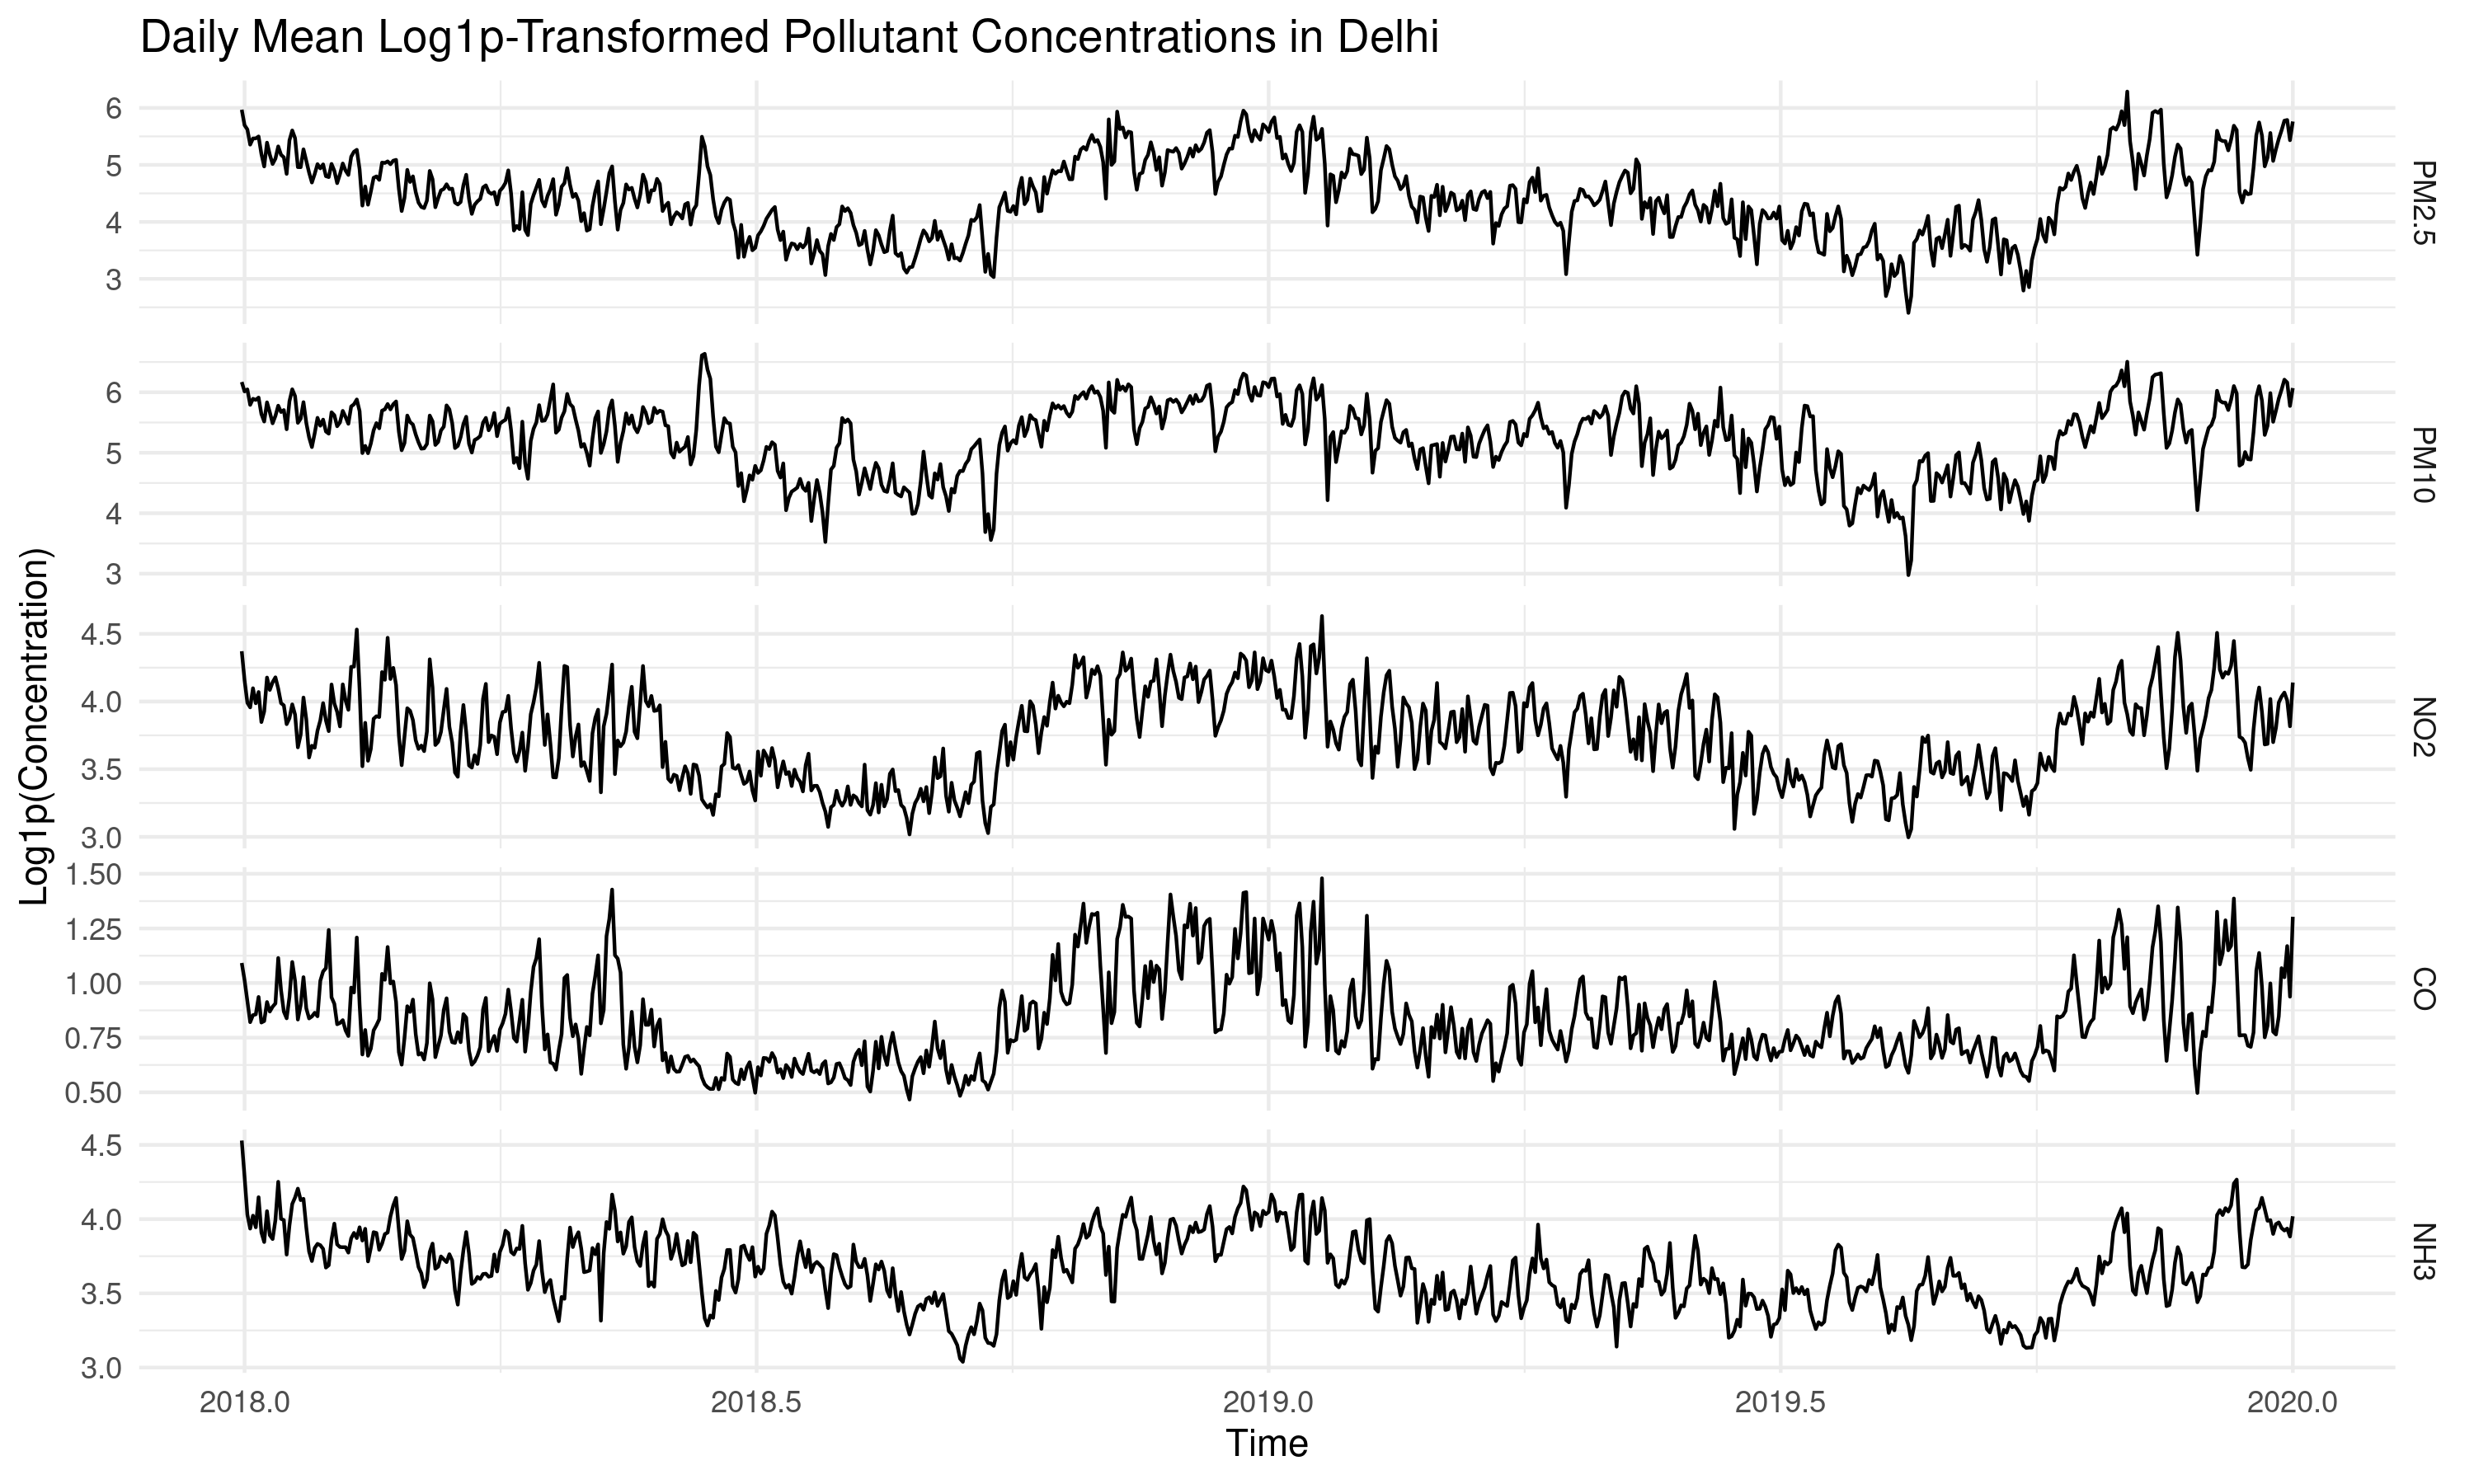
\includegraphics[width=\linewidth]{../analysis/assets/daily_ts_delhi.png}
    \caption{Daily Mean Log1p-Transformed Pollutant Concentrations in Delhi (2018-2019).}
    \label{fig:daily_ts_delhi}
\end{figure*}

\subsubsection{Correlation Insights}
The correlation matrix for the daily log1p-transformed pollutants in Delhi is shown in Figure~\ref{fig:corrplot_delhi}. All pollutants exhibit moderate to strong positive correlations with each other. A very strong positive correlation is observed between $\text{PM}_{2.5}$ and $\text{PM}_{10}$ (0.93), which is expected as $\text{PM}_{2.5}$ is a fraction of $\text{PM}_{10}$. Other notable positive correlations exist between $\text{NO}_2$ and CO (0.86), and $\text{PM}_{2.5}$ with CO (0.80) and $\text{NO}_2$ (0.84). These correlations suggest strong interdependencies between the pollutants.

\begin{figure}[ht]
    \centering
    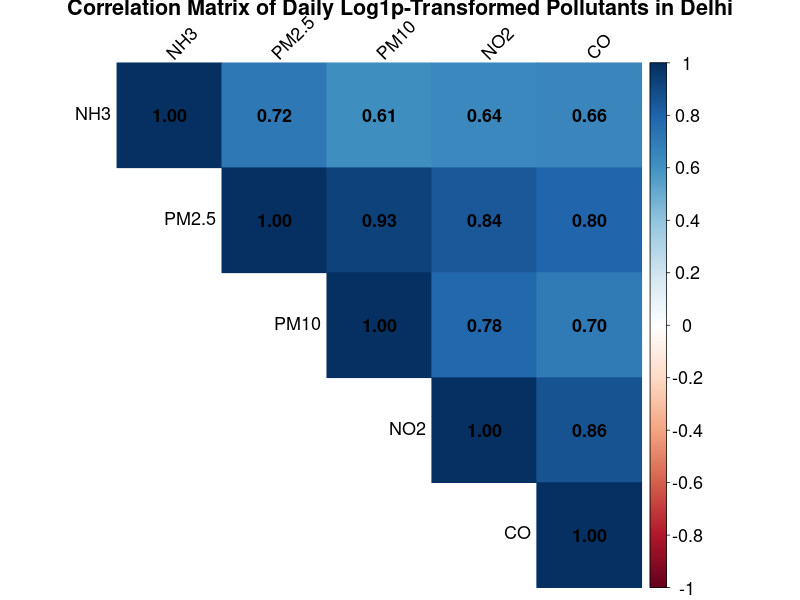
\includegraphics[width=0.8\linewidth]{../analysis/assets/corrplot_delhi.png}
    \caption{Correlation Matrix of Daily Log1p-Transformed Pollutants in Delhi (2018-2019). Numerical values represent Pearson correlation coefficients.}
    \label{fig:corrplot_delhi}
\end{figure}

\subsection{Stationarity Analysis}
Augmented Dickey-Fuller (ADF) tests were performed on the daily log1p-transformed series for each pollutant in Delhi. The results are summarized in Table~\ref{tab:adf_results}.
For all five pollutant series, the ADF test statistic was significantly lower than the 1\% critical value, leading to the rejection of the null hypothesis. Thus, all series ($\text{PM}_{2.5}$, $\text{PM}_{10}$, $\text{NO}_2$, CO, $\text{NH}_3$) were found to be stationary, I(0), at the 5\% significance level after log1p transformation and daily aggregation. This allows for the direct application of VAR and VARMA models without further differencing.

\begin{table}[hbt]
\caption{ADF Test Results for Daily Log1p-Transformed Pollutants in Delhi (Lags by AIC).}
\centering
\begin{tabular}{lccc}
\toprule
Pollutant & Test Statistic & Approx. p-value & Stationary \\
\midrule
$\text{PM}_{2.5}$ & -5.874 & $<$0.01 & TRUE \\
$\text{PM}_{10}$  & -7.268 & $<$0.01 & TRUE \\
$\text{NO}_2$    & -7.986 & $<$0.01 & TRUE \\
CO             & -8.681 & $<$0.01 & TRUE \\
$\text{NH}_3$    & -7.559 & $<$0.01 & TRUE \\
\bottomrule
\end{tabular}
\label{tab:adf_results}
\end{table}

\subsection{VAR Model Analysis}
Given the stationarity of the series, a Vector Autoregression (VAR) model was fitted on the log1p-transformed daily mean pollutant concentrations directly.

\subsubsection{Lag Order Selection}
The optimal lag order $p$ for the VAR model was determined using various information criteria on the daily data for Delhi, with a maximum lag of 30 considered. The results are shown in Table~\ref{tab:var_lag_selection}. AIC and FPE suggested $p=4$, HQ suggested $p=2$, and SC suggested $p=1$. Using the AIC, a lag order of $p=4$ was selected for the VAR model.

\begin{table}[hbt]
\caption{VAR Lag Order Selection Criteria for Daily Data (Delhi).}
\centering
\begin{tabular}{lc}
\toprule
Criterion & Selected Lag ($p$) \\
\midrule
AIC(n)    & 4 \\
HQ(n)     & 2 \\
SC(n)     & 1 \\
FPE(n)    & 4 \\
\bottomrule
\end{tabular}
\label{tab:var_lag_selection}
\end{table}

\subsubsection{VAR(4) Model Estimation}
A VAR(4) model was estimated using the five log1p-transformed daily pollutant series. The model summary indicated good overall fit, with high R-squared values for each equation (between 0.704 to 0.835). The roots of the characteristic polynomial were all less than 1 (largest was 0.9689), indicating that the estimated VAR(4) model is stable. The residuals showed some contemporaneous correlation (e.g., correlation of 0.91 between $\text{PM}_{2.5}$ and $\text{PM}_{10}$ residuals).

\subsubsection{Granger Causality}
Granger causality tests were performed based on the VAR(4) model to investigate predictive relationships. The results (Table~\ref{tab:granger_results}) indicate significant causal linkages, with all pollutants except CO showing significant Granger causality towards the other pollutants. Notably, $\text{PM}_{2.5}$ and $\text{NH}_3$ had the most significant Granger causality towards other pollutants.

\begin{table}[hbt]
\caption{Granger Causality Test Results (Based on VAR(4) model). Shows $p$-values for the F-test.}
\centering
\begin{tabular}{lc}
\toprule
Granger Causality & $p$-value \\
\midrule
$\mathrm{PM}_{2.5} \rightarrow$ Other Pollutants & $4.80 \times 10^{-5}$ \\
$\mathrm{PM}_{10} \rightarrow$ Other Pollutants & $9.81 \times 10^{-4}$ \\
$\mathrm{NO}_{2} \rightarrow$ Other Pollutants & $0.0327$ \\
$\mathrm{CO} \rightarrow$ Other Pollutants & $0.174$ \\
$\mathrm{NH}_{3} \rightarrow$ Other Pollutants & $8.56 \times 10^{-7}$ \\
\bottomrule
\end{tabular}
\label{tab:granger_results}
\end{table}

\subsubsection{Impulse Response Functions (IRFs)}
IRFs were analyzed to understand the dynamic response of each pollutant to a shock in another. Figure~\ref{fig:irf_no2_others} illustrates the response of $\text{PM}_{10}$, $\text{NO}_2$, CO, and $\text{NH}_3$ to a shock in $\text{PM}_{2.5}$. A positive shock to $\text{NO}_{2}$ leads to an immediate positive response in CO and $\text{NH}_{3}$, which lasts for 3 days. The responses of $\text{PM}_{2.5}$ and $\text{PM}_{10}$ to a $\text{NO}_{2}$ shock are also positive, but they only appear after a lag of 1 day. These IRFs die out over time.

\begin{figure*}[ht]
    \centering
    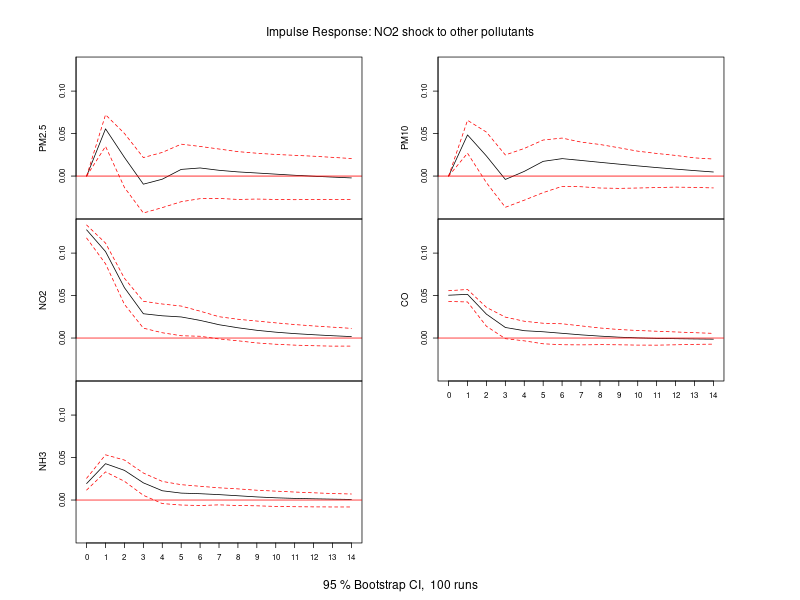
\includegraphics[width=\linewidth]{../analysis/assets/irf_no2_others.png}
    \caption{Impulse Response of Other Pollutants to a 1 SD Shock in $\text{NO}_{2}$ (log1p-transformed, daily data for Delhi, VAR(4) model). Dashed lines represent 95\% confidence intervals.}
    \label{fig:irf_no2_others}
\end{figure*}

\subsubsection{Forecast Error Variance Decomposition (FEVD)}
FEVD was used to quantify the proportion of the forecast error variance of each pollutant attributable to its own shocks versus shocks from other pollutants over a 10-day time horizon. The results plot in (Figure~\ref{fig:fevd_delhi}) show that a large portion of all pollutants' forecast error variance is explained by their own shocks, or by $PM_{2.5}$. This is probably due to the high correlations between $PM_{2.5}$ and all other pollutants. Interestingly, $NO_{2}$ also contributes significantly to the forecast error variance of $CO$. For example, at a 10-day horizon, 17.8\% of the forecast error variance of $CO$ is explained by $NO_{2}$ shocks.

\begin{figure*}[ht]
    \centering
    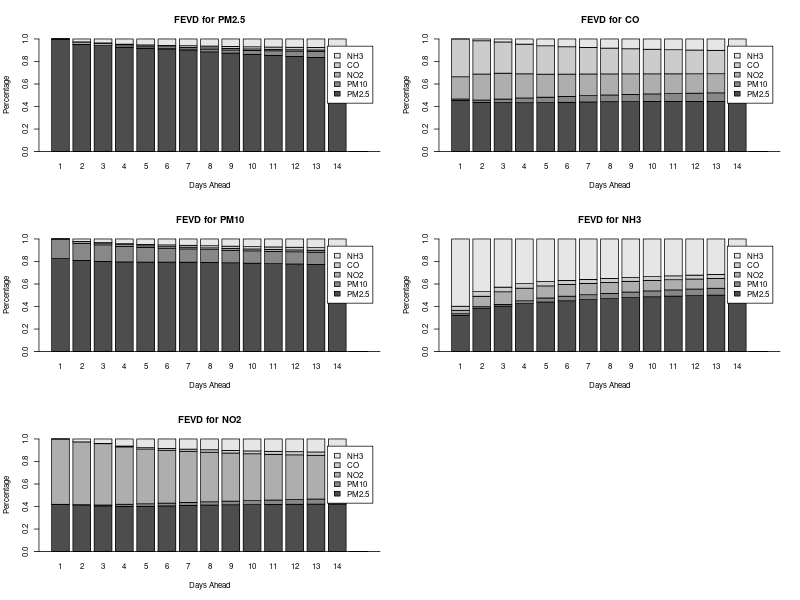
\includegraphics[width=\linewidth]{../analysis/assets/fevd_delhi.png}
    \caption{Forecast Error Variance Decomposition (FEVD) of Daily Log1p-Transformed Pollutants in Delhi (VAR(4) Model).}
    \label{fig:fevd_delhi}
\end{figure*}

\subsection{VARMA Model Analysis}
A VARMA(1,1) model was also estimated for the five log1p-transformed daily pollutant series for Delhi using the \texttt{MTS} package. This choice of (1,1) for (p,q) was illustrative, as exhaustive order selection for VARMA models is computationally intensive. Furthermore, tests with larger $p$ and $q$ values caused convergence issues. The VARMA(1,1) model was fitted to the data, and the results were compared with the VAR(4) model.

\subsection{Forecasting Evaluation}
The dataset was split into a training period (first 718 days) and a testing period (14 days). Both VAR(4) and VARMA(1,1) models were trained on the training data, and 14-day ahead forecasts were generated for the test period. The Root Mean Squared Error (RMSE) for all five pollutant forecasts was used for comparison.

The RMSE results are presented in Table~\ref{tab:rmse_comparison}. The VARMA(1,1) model showed lower RMSE for all five pollutants' forecasts compared to the VAR(4) model on the test set. This suggests that for this particular dataset and forecast horizon, the VARMA(1,1) model provided more accurate point forecasts, indicating that the inclusion of moving average terms improved the model's performance.

\begin{table}[hbt]
\caption{RMSE Comparison for 14-Day Ahead Pollutant Forecasts (Log1p-transformed scale) on the Test Set.}
\centering
\begin{tabular}{lccccc}
\toprule
Model        & $\text{PM}_{2.5}$ & $\text{PM}_{10}$ & $NO_2$ & $CO$ & $NH_3$ \\
\midrule
VAR(4)       & 0.721 & 0.543 & 0.179 & 0.202 & 0.150 \\
VARMA(1,1)   & 0.605 & 0.446 & 0.169 & 0.189 & 0.142 \\
\bottomrule
\end{tabular}
\label{tab:rmse_comparison}
\end{table}

Figure~\ref{fig:var_forecast_delhi} shows the 14-day ahead forecasts from the VAR(4) model (trained on the full dataset for illustrative purposes) for all five pollutants in Delhi. The forecasts tend to revert to the mean of the series, with widening confidence intervals as the horizon increases.

\begin{figure*}[ht]
    \centering
    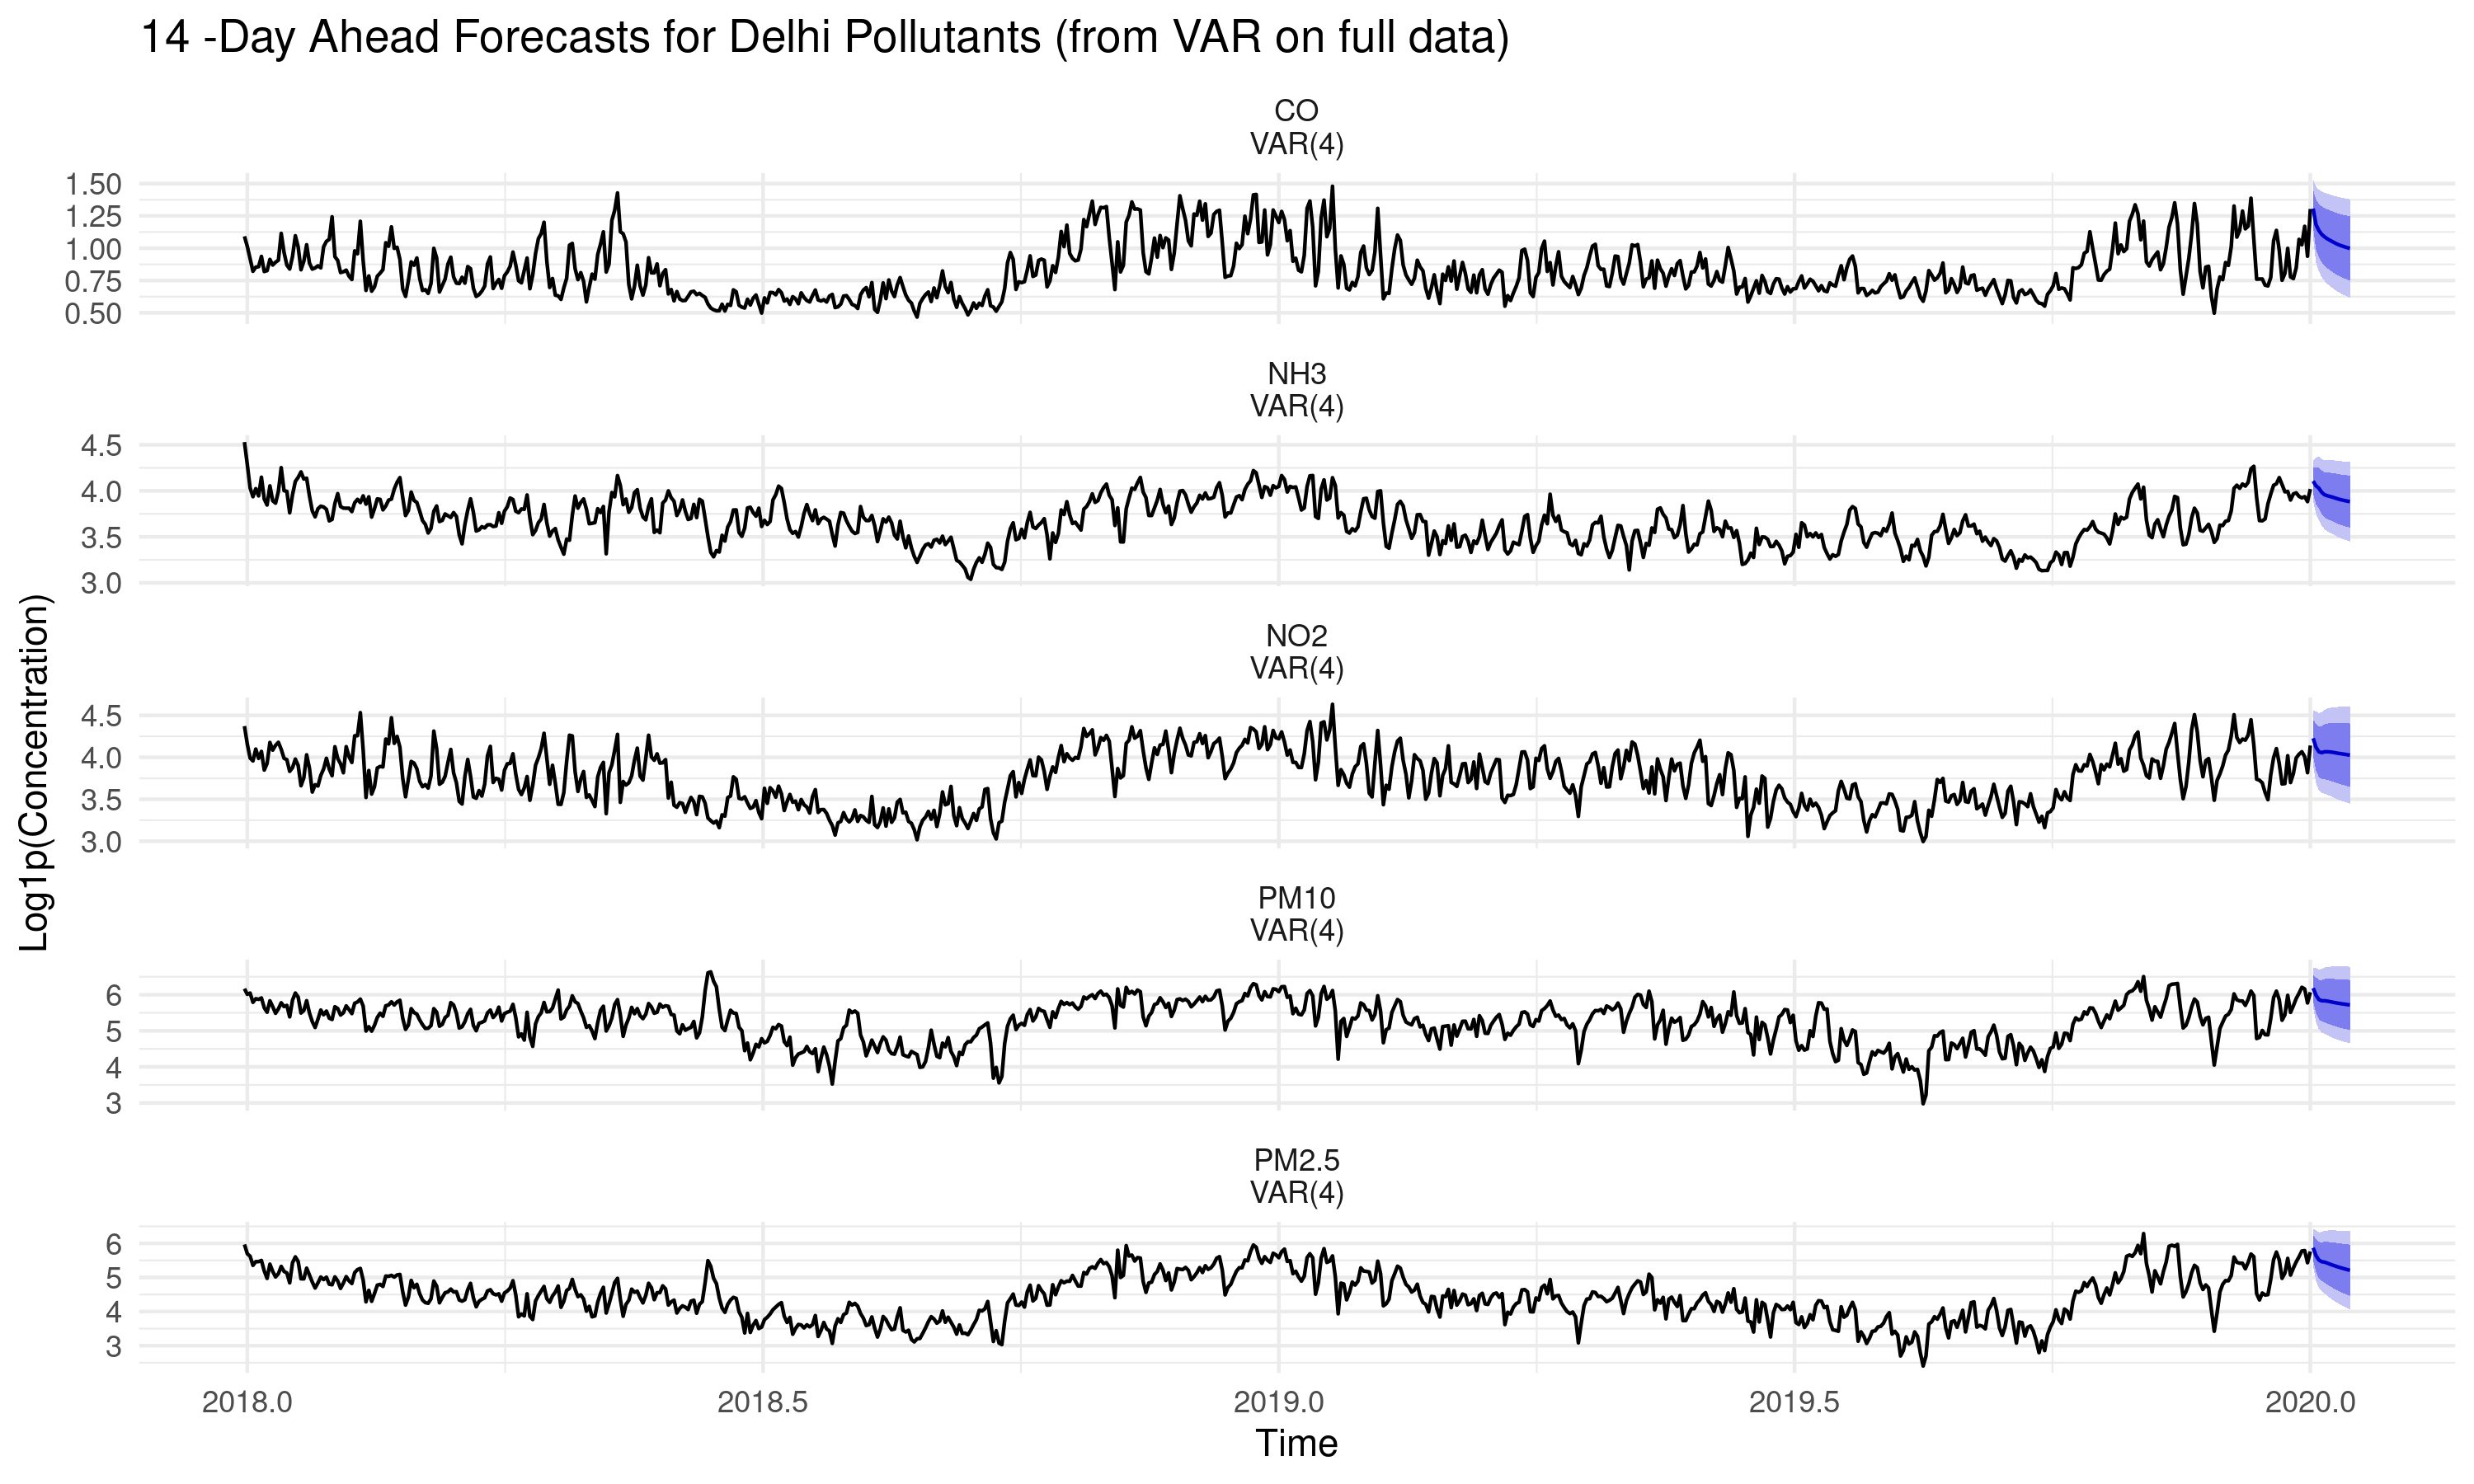
\includegraphics[width=\linewidth]{../analysis/assets/var_forecast_delhi.png}
    \caption{14-Day Ahead Forecasts for Delhi Pollutants from VAR(4) Model (Trained on Full Daily Data). Point forecasts are shown with 80\% and 95\% confidence intervals.}
    \label{fig:var_forecast_delhi}
\end{figure*}


%------------------------------------------------

\section{Conclusion}

This study investigated the multivariate dynamics of five key air pollutants ($\text{PM}_{2.5}$, $\text{PM}_{10}$, $\text{NO}_2$, CO, and $\text{NH}_3$) daily concentrations in Delhi, India, for the time period 2018-2019. After log1p transformation and aggregation to daily mean concentrations, all pollutant series were found to be stationary, I(0).

Vector Autoregressive (VAR) and Vector Autoregressive Moving Average (VARMA) models were fit to capture the interdependencies. The optimal lag order, based on the AIC criterion, was determined to be 4 for the VAR model. Granger causality tests of the VAR model confirmed significant predictive relationships. Impulse Response Functions (IRFs) showed that shocks to one pollutant, particularly $\text{NO}_{2}$, have a small positive effects on all others. Forecast Error Variance Decomposition (FEVD) indicated that a large portion of the forecast error variance for all pollutants is explained by their own shocks and by $\text{PM}_{2.5}$.

In terms of forecasting performance for the pollutants over a 14-day horizon on a small held-out test set, a VARMA(1,1) model outperformed the VAR(4) model on all pollutants, with lower RMSE values. This suggests that the inclusion of moving average terms can enhance forecast accuracy for this pollutant.

The findings demonstrate the complex, interconnected nature of air pollution in Delhi. The multivariate framework used in this study provides a valuable method for understanding these dynamics and generating forecasts.

Limitations of this study include the focus on a single city, the specific set of pollutants, and the use of linear models. Daily aggregation, while reducing noise, might obscure some hourly dynamics. Future research could extend this analysis by exploring spatial dependencies across multiple cities, removing seasonal effects, using more granular hourly data, and incorporating additional pollutants. Such extensions could provide an even more comprehensive understanding of air pollution dynamics in India.

%----------------------------------------------------------------------------------------
%   REFERENCE LIST
%----------------------------------------------------------------------------------------
\bibliographystyle{unsrt}

\begin{thebibliography}{9}

\bibitem{aladag2021}
Aladağ, E. (2021). \textit{Forecasting of Particulate Matter with a Hybrid ARIMA Model Based on Wavelet Transformation and Seasonal Adjustment}. Urban Climate. \url{https://doi.org/10.1016/j.uclim.2021.100930}.

\bibitem{hajmohammadi2021}
Hajmohammadi, H. and Heydecker, B. (2021). \textit{Multivariate time series modelling for urban air quality}. Urban Climate. \url{https://doi.org/10.1016/j.uclim.2021.100834}.

\bibitem{sethi2020}
Sethi, J.K. and Mittal, M. (2020). \textit{Analysis of Air Quality using Univariate and Multivariate Time Series Models}. \url{https://doi.org/10.1109/Confluence47617.2020.9058303}.

\bibitem{RCoreTeam2025}
R Core Team (2025). \textit{R: A Language and Environment for Statistical Computing}. R Foundation for Statistical Computing, Vienna, Austria. \url{https://www.R-project.org/}.

\bibitem{dplyr}
Wickham, H., François, R., Henry, L., Müller, K. and Vaughan, D. (2023). \textit{dplyr: A Grammar of Data Manipulation}. R package version 1.1.4. \url{https://CRAN.R-project.org/package=dplyr}.

\bibitem{ggplot2}
Wickham, H. (2016). \textit{ggplot2: Elegant Graphics for Data Analysis}. Springer-Verlag New York. \url{https://ggplot2.tidyverse.org}.

\bibitem{tidyr}
Wickham, H., Vaughan, D., Girlich, M. (2024). \textit{tidyr: Tidy Messy Data}. R package version 1.3.1, \url{https://CRAN.R-project.org/package=tidyr}.

\bibitem{forecast}
Hyndman, R., Athanasopoulos, G., Bergmeir, C., Caceres, G., Chhay, L., O'Hara-Wild, M., Petropoulos, F., Razbash, S., Wang, E., Yasmeen, F. (2025). \textit{forecast: Forecasting functions for time series and linear models}. R package version 8.24.0. \url{https://pkg.robjhyndman.com/forecast/}.

\bibitem{urca}
Pfaff, B. (2008). \textit{Analysis of Integrated and Cointegrated Time Series with R}. Second Edition. Springer, New York. ISBN 0-387-27960-1

\bibitem{vars}
Pfaff, B. (2008). \textit{VAR, SVAR and SVEC Models: Implementation Within R Package vars}. Journal of Statistical Software, 27(4). \url{https://www.jstatsoft.org/v27/i04/}.

\bibitem{MTS}
Tsay, R. S., Wood, D., Lachmann, J. (2022). \textit{MTS: All-Purpose Toolkit for Analyzing Multivariate Time Series (MTS) and Estimating Multivariate Volatility Models}. R package version 1.2.1. \url{https://CRAN.R-project.org/package=MTS}.


\end{thebibliography}

%----------------------------------------------------------------------------------------

\end{document}